% \documentclass[10pt, a4paper]{amsart}
\documentclass[%
reprint,
nofootinbib,
%superscriptaddress,
%groupedaddress,
%unsortedaddress,
%runinaddress,
%frontmatterverbose,
%preprint,
%showpacs,preprintnumbers,
%nofootinbib,
%nobibnotes,
%bibnotes,
amsmath,amssymb,
aps,
%pra,
%prb,
%rmp,
%prstab,
%prstper,
%floatfix,
]{revtex4-1}
\usepackage[]{graphicx}
\usepackage{float}
\usepackage[]{hyperref}
\usepackage[]{physics}
\usepackage[]{listings}
\usepackage[T1]{fontenc}
\usepackage{color}
\usepackage[]{subcaption}
\usepackage[ruled,vlined]{algorithm2e}
\usepackage{amssymb, amsmath}
\usepackage{caption}
\captionsetup{justification=raggedright,singlelinecheck=false}

\definecolor{mygreen}{rgb}{0,0.6,0}
\definecolor{mymauve}{rgb}{0.58,0,0.82}

\newcommand\todo[1]{\textcolor{red}{#1}}
\newcommand{\fracpt}{\frac{\partial}{\partial t}}
\newcommand{\fracpx}{\frac{\partial}{\partial x}}
\newcommand{\fracpy}{\frac{\partial}{\partial y}}
\newcommand{\fracpxx}{\frac{\partial^2}{\partial x^2}}
\newcommand{\fracpyy}{\frac{\partial^2}{\partial y^2}}
\newcommand{\pt}{{\partial t}}
\newcommand{\px}{{\partial x}}
\newcommand{\py}{{\partial y}}
\newcommand{\pu}{{\partial u}}
\newcommand{\dt}{{\Delta t}}
\newcommand{\dx}{{\Delta x}}
\newcommand{\dy}{{\Delta y}}

\lstset{ %
	backgroundcolor=\color{white},   % choose the background color; you must add \usepackage{color} or \usepackage{xcolor}
	basicstyle=\footnotesize,        % the size of the fonts that are used for the code
	breakatwhitespace=false,         % sets if automatic breaks should only happen at whitespace
	breaklines=true,                 % sets automatic line breaking
	captionpos=b,                    % sets the caption-position to bottom
	commentstyle=\color{mygreen},    % comment style
	deletekeywords={...},            % if you want to delete keywords from the given language
	escapeinside={\%*}{*)},          % if you want to add LaTeX within your code
	extendedchars=true,              % lets you use non-ASCII characters; for 8-bits encodings only, does not work with UTF-8
	frame=single,	                   % adds a frame around the code
	keepspaces=true,                 % keeps spaces in text, useful for keeping indentation of code (possibly needs columns=flexible)
	keywordstyle=\color{blue},       % keyword style
	language=c++,                    % the language of the code
	otherkeywords={*,...},           % if you want to add more keywords to the set
	rulecolor=\color{black},         % if not set, the frame-color may be changed on line-breaks within not-black text (e.g. comments (green here))
	showspaces=false,                % show spaces everywhere adding particular underscores; it overrides 'showstringspaces'
	showstringspaces=false,          % underline spaces within strings only
	showtabs=false,                  % show tabs within strings adding particular underscores
	stepnumber=2,                    % the step between two line-numbers. If it's 1, each line will be numbered
	stringstyle=\color{mymauve},     % string literal style
	tabsize=2,	                     % sets default tabsize to 2 spaces
}


\begin{document}
	
\title{Diffusion Equation \\
	\normalsize{Simulating the diffusion equation in 1 and 2 dimensions} \\
	\hrulefill\small{ FYS3150: Computational Physics }\hrulefill}

\author{Sigurd Sandvoll Sundberg}\homepage{https://github.com/SigurdSundberg/FYS3150}

\affiliation{%
	Department of Geosciences, University of Oslo\\
}%

\date{\today}

\begin{abstract} %0
	We reviewed different finite-difference schemes for solving one- and two-dimensional diffusion equation, including a mathematical analysis of their truncation error and constraints put on $\dx$ and $\dt$. The upper bound of $\alpha = \dt/\dx^2$, using von Neumann stability analysis and spectral analysis of a matrix. For the one-dimensional explicit scheme, this upper bound was found to be $\alpha = 1/2$ and for the two-dimensional scheme we have $\alpha = 1/4$. Whilst for the implicit schemes, they where found to be unconditionally stable, however no numerical analysis was done. We also found that the one-dimensional explicit scheme performed better than both the explicit schemes, having a faster convergence. Whilst for the two implicit schemes, the Crank-Nicholson scheme performed significantly better than the backward Euler at approximating the closed-form solutions. An attempt at finding the closed-form solutions for both spatial dimensions was done, with the one-dimensional closed-form solution, matching our analytical solution. The two-dimensional closed-form solution did not created the expected results from the analysis of the problem, and further study of the implementation and closed-form solutions could be interesting for further projects. In addition to study of implicit schemes for solving the two-dimensional diffusion equation and the stability and error of the schemes.
	
\end{abstract}

\maketitle 

\section{Introduction} %0
Partial differential equations plays a large part numerous branches of the natural sciences and even social sciences. In this article, the diffusion equation is of interest, modeling everything from trace diffusion in standing water to radioactive heating of the mantel. The vast majority of these process do not allow themselves to be solved analytical, forcing us to adapt to the use of numerical solvers to tackle and study these problems. Especially for studying system which we have a hard time, or which could be impossible to gather accurate data throughout the entire system. Establishing functioning numerical methods for solving problems which we have no analytical solution, by first studying problems we have an analytical solution for, is key to for having a greater understanding of the nature around us.

We will review three finite difference schemes for solving the one-dimensional diffusion equation. One explicit method in the forward Euler and two implicit methods, the backward Euler and the Crank-Nicholson scheme. Through the use of the so-called $\theta$-rule, based on Taylor expansions, we will derive the different methods, including short analysis of the constraint put on $\dt$ and $\dx$ in the different scheme. We will also look at the mathematical truncation error of the finite difference schemes and the absolute error, also known as the convergence of the different schemes. Before we extend our problem to two-dimensions, using the explicit scheme for which the same derivation is performed. We also try to find closed-form solutions for both the one-dimensional and two-dimensional case. 

\section{Theory} %0
The typical form for the one dimensional diffusion equation for a homogeneous medium is given by 
\begin{equation}\label{eq:Standard diffusion equation}
	\frac{\partial^2 }{\partial x^2}u = D\frac{\partial}{\partial t}u,\, x\in[0,L],\, t\in[0,T],
\end{equation}
where $D$ the diffusion coefficient. D typically is a conglomerate of other physical values for the problem at hand.

The multi-dimensional extension of the diffusion equation takes the form 
\begin{equation}\label{eq Multi dim diffusion equation}
	\frac{\partial}{\partial t}\vec{u} = D\Delta \vec{u}, \, \vec{u} = (x,y,z)\in\Omega,\, t\in(0,T].
\end{equation}
\subsection{Scaling the Diffusion Equation}
We can further simplify the diffusion equation by scaling it. Making a dimensional problem into a dimensionless problem, where vastly different systems can be boiled down the same equation. Following the scaling proposed in Langtangen's book on \textit{Scaling of Differential Equations} \cite{Langtangen2016}, using the dimensionless variables 
\begin{equation}
	\hat{x} = \frac{x}{x_c},\, \hat{t} = \frac{t}{t_c}, \, \hat{u}=\frac{u}{u_c}. 
\end{equation}
If we insert the dimensionless variables denoted $\hat{x}$, we get 
\begin{equation}
	\frac{\partial}{\partial \hat{t}}\hat{u} = \frac{t_cD}{L^2}\frac{\partial^2}{\partial x^2}\hat{u}, \, \hat{x}\in(0,1), \, \hat{t}\in(0,\hat{T} = T/t_c].
\end{equation}
If we chose $t_cD/L^2 = 1$, it results in $t_c = L^2/D$, and our scaled diffusion equations then takes the form 
\begin{equation}\label{eq: Scaled diffusion equation}
	\fracpt u = \fracpxx u.
\end{equation}
This equation is the one we will use from now on. 

The multi-dimensional form follows almost the same scaling and the final form just adds the other dimensional terms. 
\subsection{Establishing the Problem}
Our dimensionless problem follows equation \eqref{eq: Scaled diffusion equation} with $t>0$, $x\in[0,L]$. This could be the temperature gradient of a rod of length L heated from one end. 
The initial conditions of the problem is given by 
\begin{equation}
	u(x,0) = 0, \quad 0 < x < L
\end{equation}
with $L = 1$, the length of the $x-region$. The boundary conditions are given as 
\begin{equation}
	\begin{split}
	u(0,t) &= 0, \quad t\geq 0,\\
	u(L,t) &= 1, \quad t\geq 0.
	\end{split}
\end{equation}

We can rewrite this as follows which will be useful for later
\begin{equation}\label{eq Adapted problem}
	v(x,t) = u(x,t) + f(x) = 0.
\end{equation}
This gives us a new set of boundary and initial conditions given as 
\begin{equation}\label{eq new boundaries}
	\begin{split}
		v(x,0) &= u(x,0) + f(x) = f(x) \\
		v(0,t) &= u(0,t) + f(0) = 0 \\
		v(L,t) &= u(L,t) + f(L) = 0 
	\end{split}
\end{equation}

To determine our function require new initial condition $f(x)$ we can take the initial conditions from \eqref{eq new boundaries} which gives us 
\begin{equation}
	\begin{split}
		v(0,t) = u(0,t) + f(0) = 0 &\rightarrow f(0) = 0\\
		v(L,t) = u(L,t) + f(L) = 0 &\rightarrow f(L) = -1.
	\end{split}
\end{equation}
From this we require 
\begin{equation}
	\fracpxx f = 0,
\end{equation}
with the above constraints on $f(x)$. From this we find that 
\begin{equation}
	f(x) = c_1 + c_2x,
\end{equation}
applying the constraints on $f(x)$ we find 
\begin{equation}
	\begin{split}
		f(0) = 0 &\rightarrow c_1 = 0\\
		f(L) = -1 &\rightarrow c_2 = -\frac{1}{L}
	\end{split}
\end{equation}
so we have 
\begin{equation}\label{eq f(x)}
	f(x) = -\frac{x}{L}.
\end{equation}

\subsection{Extending to Two Dimensions}
There are multiple ways of extending the problems to two dimensions. One way would be to think of an infinitely wide square, i.e. we have no fluxes to either side\footnote{The mantel of the earth is such a prospect or the atmosphere.}. For this we can fix two temperatures at the two remaining edges in short giving us a problem where we have two set of Dirichlet boundary conditions and two edges with Neumann boundary conditions. 

By simply just adding a term to our one dimensional diffusion equation, we then have 
\begin{equation}\label{eq diffusion 2d}
	\fracpxx u + \fracpyy u = \fracpt u.
\end{equation}

If we set our dimensions of the square in question to $x,y\in [0,L]$, we can have 
\begin{equation}
	\begin{split}
		u(0,y,t) &= 0\\
		u(L,y,t) &= 1\\
		\frac{\partial}{\partial y}u(x,0,t) &= 0\\
		\frac{\partial}{\partial y}u(x,L,t) &= 0
	\end{split}
\end{equation}

Another way is to only use Neumann boundaries, or only Dirichlet boundaries, the options and the systems you can simulate with different choices of boundaries are plentiful. Some examples can be a metal sheet with no fluxes at the edges and a heat source at a specific point, or the heat evolution in a square with three edges at the same temperatures and the last edge at a different temperature. As mention the system we can study are plentiful. 

In this article we will use the above mentioned boundary conditions, and they will also be used in finding the analytical solutions for the two dimensional problem. 


\subsection{Analytical Solution}
For many numerical problems finding closed-form solution are not possible and comparing a numerical scheme to a closed-form solution is a good way to check whether the scheme is implemented correctly or not. This can serve as a baseline for studying how different algorithms differ and what algorithm is the correct choice of the problem, balancing between implementation time and accuracy. 

The one- and two-dimensional diffusion equation do have closed-form solution which we can use to study the error of our scheme compared to the analytical solutions. 
\subsubsection{One-Dimensional}
Starting off with the one-dimensional case we have the equation 
\begin{equation}
	\fracpt u = \fracpxx u. 
\end{equation}
Studying the equation \eqref{eq Adapted problem} with the new boundary conditions found in \ref{eq new boundaries} we start off by using method of separation of variables. We start off with 
\begin{equation}
	v(x,t) = F(x)G(t),
\end{equation}
inserting into the equation \eqref{eq: Scaled diffusion equation} it results in 
\begin{equation}
	\frac{F''}{F} = \frac{G'}{G}.
\end{equation}
This equation should hold for all $x$ and $t$. So we must require that the right-hand side and left-hand side to be equal to a constant. Lets call this constant $-\lambda^2$. This gives us two differential equations
\begin{equation}
	F'' + \lambda^2 F = 0, \quad G' = -\lambda^2 G,
\end{equation}
with general solutions
\begin{equation}
	F(x) = A\sin(\lambda x)+ B\cos(\lambda x), \quad G(t) = Ce^{-\lambda^2 t}.
\end{equation}
Using our new boundary conditions \eqref{eq new boundaries}, we require that $B=0$ and $\lambda = n\pi/L$. 

This gives us a set of solution on the form 
\begin{equation}
	v(x,t) = \sum_{n=1}^\infty A_n\sin(n\pi x/L)e^{-n^2\pi^2 t/L^2}.
\end{equation}
We can determine the coefficient $A_n$ using the initial condition. We require 
\begin{equation}
	v(x,0) = f(x) = \sum_{n=1}^\infty A_n\sin(n\pi x/L).
\end{equation}

The coefficient $A_n$ is the Fourier coefficients for the function $f(x)$\cite{morten}, because of this, $A_n$ is given by 
\begin{equation}
	A_n = \frac{2}{L}\int_0^L f(x)\sin(n\pi x/L)dx.
\end{equation}
The integrated form is 
\begin{equation}
	A_n = \frac{2\pi n \cos(\pi n) - 2\sin(\pi n)}{\pi^2n^2}.
\end{equation}

So our analytical solution is given by 
\begin{equation}\label{eq analytical 1d}
	v(x,t) = \sum_{n=1}^\infty \frac{2\pi n \cos(\pi n) - 2\sin(\pi n)}{\pi^2n^2}\sin(n\pi x/L)e^{-n^2\pi^2 t/L^2}.
\end{equation}

\subsubsection{Two-Dimensional}
The two-dimensional case follows a similar approach to that of the 1-dimensional solution and we will simply state the result of the closed-form solution. 
\begin{equation}
	v(x,y,t) = 
		\sum_{n = 1}^{\infty}\sum_{m=1}^{\infty}\left(A_{nm}\right)\sin\left(\frac{n\pi x}{L}\right)\cos\left(\frac{n\pi y}{L}\right)e^{-\lambda_{nm}t}
\end{equation}
where we have 
\begin{equation}
	\begin{split}
		A_{nm} &= \frac{4\left( n\pi\cos(n\pi) - \sin(n\pi)\right)\sin(n\pi)}{n^3\pi^3}\\
		\lambda_{nm} &= \pi^2\left(\frac{n^2+m^2}{L^2}\right)
	\end{split}
\end{equation}
For the full derivation see Appendix \ref{app 2DA}.
\subsection{Discretization}
To apply numerical solutions to a continuous problem, we are required to discretize the continuous equations. Taking $x, t, u(x,t)$ as a baseline example we get 
\begin{equation}
	\begin{split}
		x \rightarrow x_i &\in [x_0,x_1,\dots,x_i,\dots,x_{n+1}]\\		
		t \rightarrow t_j &\in [t_0,t_1,\dots,t_j,\dots,t_{n}]\\
		u(x,t)\rightarrow u(x_i,t_j) = u_i^j &\in [u_0^j,u_1^j,\dots,u_i^j,\dots,u_{n+1}^j]
	\end{split}
\end{equation}
With $j$ denoting time index of $u$, and $i$ the spatial index. 
The grid-point $x_i = ih$, with $h = (x_{max} - x_{min})/(n+1)$. 

This notation will be used when deriving the different numerical schemes. 
\subsection{$\theta$-Rule}
Taking the continuous equation \eqref{eq: Scaled diffusion equation}, expanding it using forward in time, centered in space for transforming the continuous equation to a discretized version. We can write this as 
\begin{equation}\label{eq theta}
	\begin{split}
			\frac{\theta}{\Delta x^2}\left(u_{i-1}^j - 2u_i^j +  u_{i+1}^j\right) + \frac{1 - \theta}{\Delta x^2}\left(u_{i+1}^{j-1} - 2u_i^{j-1} + u_{i-1}^{j-1}\right)\\
			 = \frac{1}{\Delta t}\left(u_i^j - u_i^{j-1}\right).
	\end{split}
\end{equation}
From this expansion we can create different formulas depending on our choice of $\theta$.

For the following numerical methods we will be using the following Dirichlet boundary conditions
\begin{equation}
	u(0,t) = u(L,t) = 0, \quad u_0 = u_n = 0
\end{equation}
\subsection{Forward Euler}
Choosing $\theta = 0$, we obtain the forward Euler formula, 
\begin{align}
	\frac{u_i^{j+1} - u_i^j}{\dt} &= \frac{u_{i+1}^j + u_{i-1}^j - 2u_i^j}{\dx^2}\\
	u_i^{j+1} &= \alpha \left(u_{i+1}^j + u_{i-1}^j\right) + \left(1-2\alpha\right)u_i^j
\end{align}
where $\alpha = dt/dx^2$. Following the similar expansion method as used in \cite{Sigurd1}, we obtain the following matrix equation
\begin{equation}
	\mathbf{A}u^{j} = u^{j+1}
\end{equation}
with $\mathbf{A}$ for a $4\times 4$ matrix given as 
\begin{equation}\label{mat FE}
\mathbf{A} =	\begin{bmatrix}
		1-2\alpha & \alpha & 0 & 0 \\
		\alpha & 1-2\alpha & \alpha & 0 \\
		0 &	\alpha & 1-2\alpha & \alpha \\
		0 & 0 &	\alpha & 1-2\alpha
	\end{bmatrix},
\end{equation}
and 
\begin{equation}
	u^{j+1} = \begin{bmatrix}
		u^{j+1}_0\\		u^{j+1}_1 \\ u^{j+1}_2 \\u^{j+1}_3
	\end{bmatrix}, \quad 
		u^{j} = \begin{bmatrix}
		u^{j}_0\\		u^{j}_1 \\ u^{j}_2 \\u^{j}_3
	\end{bmatrix}
\end{equation}.
\subsubsection{Truncation Error}
From the Taylor expansions used to find the forward in time centered in space schemes, we know that the truncation error for the forward Euler scheme goes as $\mathcal{O}(\dx^2)$ and $\mathcal{O}(\dt)$. 
\subsubsection{Constraint}
For the forward Euler we have a fairly strict limitation on values of $\alpha$. The scheme is in other words not stable for values of $\alpha > 1/2$. This constraint comes from the study of the spectral radius of $\rho(\mathbf{A})$ of our matrix $\mathbf{A}$ satisfies the condition 
\begin{equation}
	\rho(\mathbf{A}) < 1. 
\end{equation}
The spectral radius is defined as\cite{morten}
\begin{equation}
	\rho(\mathbf{A}) = \text{max} \left\lbrace |\lambda| : \text{det}\left(\mathbf{A} - \lambda \mathcal{I}\right) = 0\right\rbrace.
\end{equation}

From this we have that if a matrix is positive definite, then the condition is always satisfied. We can rewrite $\mathbf{A}$ as 
\begin{equation}
	\mathbf{A} = \mathcal{I} - \alpha\mathbf{B},
\end{equation}
with 
\begin{equation}
	\begin{bmatrix}
		2 & -1 & 0 & 0 \\
		-1 & 2 & -1 & 0 \\
		0 &	-1 & 2 & -1 \\
		0 & 0 &	-1 & 2
	\end{bmatrix}.
\end{equation}
The eigenvalues of $\mathbf{A}$ are then given as $\lambda_i = 1 - \alpha\mu_i$, with $\mu_i$ being the eigenvalues of $\mathbf{B}$. Using the results found in \cite{morten}, we find that the eigenvalues of $\mathbf{A}$ then results in 
\begin{equation}
	-1 < 1-\alpha 2(1-\cos(\theta)) < 1, 
\end{equation}
which puts our requirement for $\alpha$ to, $\alpha < (1-\cos(\theta))^{-1}$, resulting in $\alpha < 1/2$. 


\subsection{Backward Euler}
The backward Euler formula is obtained by choosing $\theta = 1$ in equation \eqref{eq theta}, obtaining
\begin{align}
\frac{u_{i+1}^{j+1} + u_{i-1}^{j+1} - 2u_i^{j+1}}{\dx^2}&= 	\frac{u_i^{j+1} - u_i^j}{\dt} \\
	-\alpha \left(u_{i+1}^{j+1} + u_{i-1}^{j+1}\right) + \left(1+2\alpha\right)u_i^{j+1}&= u_i^j
\end{align}
where $\alpha = \dt/\dx^2$.
From this we can get the following matrix equation
\begin{equation}
	\mathbf{A}u^{j+1} = u^j
\end{equation}
expanding the equations for the backward Euler, the same was as for forward Euler. Simply by expanding it for $i=3$, we can easily see the system emerge\footnote{We will show this expansion when considering the Crank-Nicholson scheme later.}. 

Our matrix $\mathbf{A}$ would then be given by 
\begin{equation}\label{mat BE}
	\mathbf{A} =	\begin{bmatrix}
		1+2\alpha & -\alpha & 0 & 0 \\
		-\alpha & 1+2\alpha & -\alpha & 0 \\
		0 &	-\alpha & 1+2\alpha & -\alpha \\
		0 & 0 &	-\alpha & 1+2\alpha
	\end{bmatrix},
\end{equation}
and 
\begin{equation}
	u^{j+1} = \begin{bmatrix}
		u^{j+1}_0\\		u^{j+1}_1 \\ u^{j+1}_2 \\u^{j+1}_3
	\end{bmatrix}, \quad 
	u^{j} = \begin{bmatrix}
		u^{j}_0\\		u^{j}_1 \\ u^{j}_2 \\u^{j}_3
	\end{bmatrix}
\end{equation}.
\subsubsection{Truncation Error}
The truncation error here goes the same as for the forward Euler, as we are expanding our problem using the same Taylor expansion, thus we have $\mathcal{O}(\dx^2)$ and $\mathcal{O}(\dt)$.
\subsubsection{Constraint}
Following the same study of the spectral radius of $\mathbf{A}$, one can show that the constraint on $\alpha$ is unconditional, that is we can choose any value of $\alpha$ and the scheme remains stable\cite{bookA}. However it is still beneficial to choose $\alpha$, and thus $\dt\,\land\,\dx$ such that we get a good approximation.

\subsection{Crank-Nicholson}
The Crank-Nicholson scheme is obtained by choosing $\theta = 1/2$ in equation \ref{eq theta}. 
This gives us 
\begin{equation}
	\begin{split}
			\frac{u_i^{j+1} - u_i^j}{\dt} &= \frac{u_{i+1}^{j+1} + u_{i-1}^{j+1} - 2u_i^{j+1}}{2\dx^2} \\
			&+ \frac{u_{i+1}^{j} + u_{i-1}^{j} - 2u_i^{j}}{2\dx^2},
	\end{split}
\end{equation}
if we collect common terms we have 
\begin{equation}
\begin{split}
		&-\alpha\left(u_{i+1}^{j+1} + u_{i-1}^{j+1}\right) + (2+2\alpha)u_i^{j+1} \\
		&=-\alpha\left(u_{i+1}^{j} + u_{i-1}^{j}\right) + (2-2\alpha)u_i^{j} 
\end{split}
\end{equation}
using $\alpha = \dt /\dx^2$. 
Expanding this for $i = 0,1,2,3$, using $u_{-1} = 0$ and $u_{4} = 0$, we have
\begin{align}
	&\begin{split}
		&-\alpha\left(u_{1}^{j+1}\right) + (2+2\alpha)u_0^{j+1} \\
		&=-\alpha\left(u_{1}^{j}\right) + (2-2\alpha)u_0^{j} 
	\end{split}\\
		&\begin{split}
		&-\alpha\left(u_{2}^{j+1} + u_{0}^{j+1}\right) + (2+2\alpha)u_1^{j+1} \\
		&=-\alpha\left(u_{2}^{j} + u_{0}^{j}\right) + (2-2\alpha)u_1^{j} 
	\end{split}\\
		&\begin{split}
		&-\alpha\left(u_{3}^{j+1} + u_{1}^{j+1}\right) + (2+2\alpha)u_2^{j+1} \\
		&=-\alpha\left(u_{3}^{j} + u_{1}^{j}\right) + (2-2\alpha)u_2^{j} 
	\end{split}\\
		&\begin{split}
		&-\alpha\left(u_{2}^{j+1}\right) + (2+2\alpha)u_3^{j+1} \\
		&=-\alpha\left(u_{2}^{j}\right) + (2-2\alpha)u_3^{j} 
	\end{split}
\end{align}
Again we can rewrite this as a matrix equation on the form 
\begin{equation}
	\mathbf{A}u^{j+1} = \mathbf{B}u^j.
\end{equation}
Where we have 
\begin{equation}\label{mat CN1}
	\mathbf{A} = \begin{bmatrix}
		2+2\alpha & -\alpha & 0 & 0 \\
		-\alpha & 2+2\alpha & -\alpha & 0 \\
		0 &	-\alpha & 2+2\alpha & -\alpha \\
		0 & 0 &	-\alpha & 2+2\alpha
	\end{bmatrix}
\end{equation}
and 
\begin{equation}\label{mat CN2}
	\mathbf{B} = \begin{bmatrix}
		2-2\alpha & \alpha & 0 & 0 \\
		\alpha & 2-2\alpha & \alpha & 0 \\
		0 &	\alpha & 2-2\alpha & \alpha \\
		0 & 0 &	\alpha & 2-2\alpha
	\end{bmatrix}.
\end{equation}
And where we have $u^{j+1}$ and $u^j$ defined as before. 
\subsubsection{Truncation Error}
Another way to look at the Crank-Nicholson method is as a half-time step approximation, a version of the mid-point rule for integration. But using the forward and backward Euler methods to for the set of points needed. Following the methods used in \cite{Langtangen2015}, we have 
\begin{equation}
	\left[D_t u = -au\right]^{n+\frac{1}{2}},
\end{equation}
where we can add a residual term $R$, thus giving us 
\begin{equation}
	\left[D_t u_e + a\overline{u_e} = R\right]^{n+\frac{1}{2}}.
\end{equation}
where $_e$ is the exact solution, and $\overline{u_e}$ is the arithmetic mean. 
From this we have as per \cite{Langtangen2015}, 
\begin{equation}
	R^{n+\frac{1}{2}} = \left(\frac{1}{24}u'''_e(t_{n+\frac{1}{2}}) + \frac{1}{8}u''(t_n)\right)\dt^2 = \mathcal{O}(\dt^4)
\end{equation}
from this we can see that the truncation error of Crank-Nicholson method is $\mathcal{O}(\dt^2)$. For the entire derivation see \cite{Langtangen2015}.

\subsubsection{Constraint}
The constraints for the Crank-Nicholson scheme is the same as for the backwards Euler, we are\cite{bookA} free to choose $\dt$ and $\dx$ freely. 

\subsection{Forward Euler Two-Dimensions}
For solving the two dimensional diffusion equation, we have chosen to use the forward Euler method. Whilst this put restrictions on our chosen values of $\alpha$, it has the same truncation error as the backward Euler. 

Assuming a square lattice, with equal many mesh points in either direction, we can discretize equation \eqref{eq diffusion 2d}, as 
\begin{equation}\label{eq FE2D}
	u_{i,j}^{l+1} = u_{i,j}^l + \alpha\left[u_{i+1,j}^{l} + u_{i-1,j}^{l} + u_{i,j+1}^{l} + u_{i,j-1}^{l} - 4u_{i,j}^{l}\right]
\end{equation}
using the same differentiation scheme as for the one dimensional counterparts. We also have $\alpha$ given as before by $\alpha = \dt/h^2$, with $h^2 = \dx^2 = \dy^2$.  

\subsubsection{Constraint}
As is important with the forward Euler method is the constraint we have to put on $\dt$ and $\dx$. The von Neumann stability analysis of the two-dimensional heat equation, is based on studying the growth of waves\cite{MITLec14}, $e^{ikx}$. 

For two-dimensions we then have 
\begin{equation}
	u(x,y,t_n) = e^{i(k,l)\cdot\left(x\atop y\right)} = e^{ikx}\cdot e^{ily}
\end{equation}

Writing our equation \eqref{eq diffusion 2d} on a different form then equation \eqref{eq FE2D}, we have
\begin{equation}
	\begin{split}
		\frac{u_{i,j}^{l+1} - u_{i,j}^{l}}{\dt} &= \frac{u_{i+1,j}^{l} - 2u_{i,j}^{l}+u_{i-1,j}^{l}}{\dx^2} \\
		&+ \frac{u_{i,j+1}^{l} - 2u_{i,j}^{l}+u_{i,j-1}^{l}}{\dy^2}
	\end{split}
\end{equation}
which can be rewritten, using $u_{i,j}^{l} = x^{ikx}, \quad x = 0$ for the current step and $G = u_{i,j}^{l+1}$. Where $G$ is the growth factor, and if $|G(k)|<1,\,\forall k$ the scheme is stable. We then have 
\begin{equation}
	\begin{split}
		\frac{G - 1}{\dt} &= \frac{e^{ik\dx} - 	2+e^{-ik\dx}}{\dx^2} \\
		&+ \frac{e^{il\dy} - 2+e^{-il\dy}}{\dy^2}
	\end{split}
\end{equation}
this implies 
\begin{equation}
	G = 1-2\frac{\dt}{\dx^2}\left(1-\cos\left(k\dx\right)\right) - 2\frac{\dt}{\dy^2}\left(1-\cos\left(l\dy\right)\right).
\end{equation}
This has a worst case at $k\dx = \pi = l\dy$ which implies
\begin{equation}
	G = 1-4\frac{\dt}{\dx^2}-4\frac{\dt}{\dy^2},
\end{equation}
thus we have the following restriction on $\dt$
\begin{equation}
	\begin{split}
			\dt &\leq \frac{1}{2}\left(\frac{1}{\dx^2} + \frac{1}{\dy^2}\right)\\
			&= \frac{\dx^2 + \dy^2}{8} \underbrace{=}_{\dx = h = \dy} \frac{h^2}{4},
	\end{split}
\end{equation}
or $\alpha \leq 1/4$.
\section{Algorithms} %0
We assume we have vectors of length $N$, which means that we have vectors such that we have $N-2$ interior points and two fixed end points. 
\subsection{Algorithm Components}
Algorithm \ref{algo:FE}, shows the simple implementation of the forward Euler method. 
\begin{algorithm}[H]\label{algo:FE}
	\SetAlgoLined
	\caption{Forward Substitution}
	\texttt{Initialization}\\
	\For{\texttt{i = 1; i < $N$; i++}}{
			\texttt{$\hat{u}_{i} = \alpha (u_{i+1} + u_{i-1}) + eu_i$}\\
		}
\end{algorithm}
Algorithm \ref{algo:TDMA} shows the Tridiagonal Matrix algorithm, also known as the Thomas algorithm \cite{datta2010numerical}, implemented as in \cite{Sigurd1}.
\begin{algorithm}[H]\label{algo:TDMA}
	\SetAlgoLined
	\caption{Tridiagonal Matrix Algorithm}
	\texttt{Initialization}	\\
	\For{\texttt{i = 1; i < $N - 1$; i++}}{
		\texttt{$\hat{b}_i = b_i - a_{i-1}c_{i-1}/\hat{b}_{i-1}$}\\
		\texttt{$u'_i = u_i - u'_{i-1}a_{i-1}/\hat{b}_{i-1}$}\\
	}
	\texttt{$\hat{u}_n = u'_n/\hat{b}_n$}\\
	\For{\texttt{i = $N-1$; i > 0; i--}}{
		\texttt{$\hat{u} = (u'_i - \hat{u}_{i+1}c_i)/\hat{b}_i$}\\
	}
\end{algorithm}

\subsubsection{Forward Euler}
The forward Euler method for solving tridiagonal matrix equation on the form 
\begin{equation}
	u^{j+1} = \mathbf{A}u^j.
\end{equation}
We can use algorithm \ref{algo:FE}, where from the matrix form in equation \eqref{mat FE} we have $e = 1 - 2\alpha$ and $\alpha = dt/dx^2$. 
\subsubsection{Backward Euler}
The backward Euler method for solving tridiagonal matrix equations on the form 
\begin{equation}
	\mathbf{A}u^{j+1} = u^j.
\end{equation}
We can apply algorithm \ref{algo:TDMA} using $a = \alpha$ and $b = 1+2\alpha$. This comes from the matrix form in equation \eqref{mat BE}.
\subsubsection{Crank-Nicholson}
The Crank-Nicholson method for solving tridiagonal matrix equations on the form 
\begin{equation}
	\mathbf{A}u^{j+1} = \mathbf{B}u^j.
\end{equation}
To solve this equation, we can either go ahead with a matrix inversion, however as our matrices are sparse we can implement a partial approach. If we solve the right-hand side first the solve the left-hand side, we can apply both our algorithms in combination. We have 
\begin{align}
	\mathbf{A}u^{j+1} &= \mathbf{B}u^j\label{eq first}\\ 
	\mathbf{A}u^{j+1} &= u'^j \label{eq: second}
\end{align}
where we solve equation \eqref{eq first} using algorithm \ref{algo:FE} and solve our new equation \eqref{eq: second} using algorithm \ref{algo:TDMA} using the values from equations (\ref{mat CN1}, \ref{mat CN2}) for our matrices $\mathbf{A}$ and $\mathbf{B}$.

\subsection{Two-Dimensional Extension}
An implementation of equation \eqref{eq FE2D}, for the two-dimensions using the forward Euler scheme may look as
\begin{algorithm}[H]\label{algo:FE2D}
	\SetAlgoLined
	\caption{Forward Euler Two Dimensions}
	\texttt{Initialization}\\
	\For{\texttt{i = 1; i < $N$; i++}}{
		\For{\texttt{j = 1; j<$N$; j++}}{
			\texttt{$\text{Q} = \alpha\left(\mathbf{U}[i+1,j] + \mathbf{U}[i - 1,j]\right.$}\\
			\texttt{$\quad\left. + \mathbf{U}[i,j+1] + \mathbf{U}[i,j-1] - 4\mathbf{U}[i,j] \right)$}\\
			\texttt{$\mathbf{\hat{U}}[i,j] = \mathbf{U}[i,j] + \text{Q}$}\\	
		}
	}
\end{algorithm}



\section{Results} %0
\subsection{One-Dimensional Solutions}
\subsubsection{Curved}
In \autoref{fig plot1d0101} and \autoref{fig plot1d01001} a chosen time value for which the solution is still significantly curved for two different time steps. The time steps in questions is chosen by the constraint put on $\dt$ in the forward Euler scheme, by a chosen value of $\dx$. Our two chosen values of $\dx$ are $\dx = 1/10$ and $\dx = 1/100$, this corresponds to \autoref{fig plot1d0101} and \autoref{fig plot1d01001}, respectively. The corresponding $\dt$ values are then given as $\dt = 0.005$, and $\dt = 0.00005$, respectively. 


A good separation of the different curves is visible for the largest time step, but separating the lines for the smaller time step is difficult. 
\subsubsection{Linear}
In \autoref{fig plot1d0401} and \autoref{fig plot1d04001} a chosen time value for which the solution is almost linear for the same two time steps as earlier. 

Almost no difference in the methods are visible in the graphs, all the methods are converging relatively quickly. 
\subsection{Error}
\subsubsection{Curved}
In \autoref{fig error0101} and \autoref{fig error01001} the absolute error between the analytical solution and the numerical estimate for the curved solutions. The convergence for the different methods refer to how close they are to a straight line, thus we can see that the forward Euler method converges the quickest, whilst the backward Euler is fairly slow. 
\subsubsection{Linear}
In \autoref{fig error0401} and \autoref{fig error04001} the absolute error between the analytical solution and the numerical estimate for the almost linear solutions. The convergence is again given by the same, and we can again see that the forward Euler converges the quickest whilst backward Euler is is slower. 
\subsection{Two-Dimensional Solutions}
In \autoref{fig 2d1} we see the steady state solution for our two-dimensional scheme. Which shows a even gradient on the color mapping of the solution, whilst in \autoref{fig 2d4} we see a sharper gradient and a larger area for which we have a close to uniform solution. This also coincides with our results for the one-dimensional case, where we have a gradual evolution of the system, so this result in two-dimensions shows a significantly curved solution. 

\begin{figure}
	\centering
	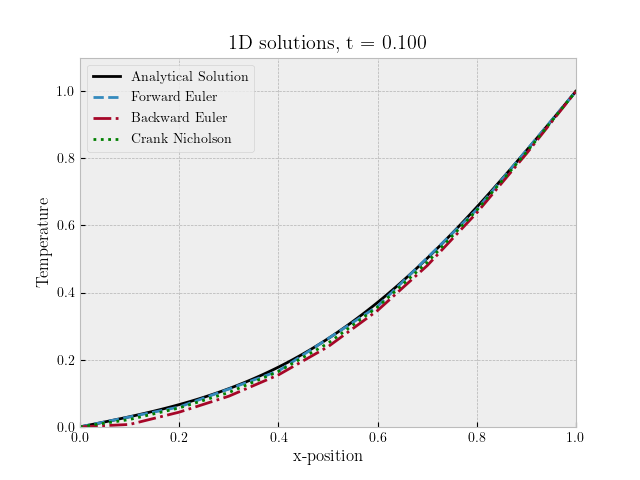
\includegraphics[width=0.95\linewidth]{./figures/plot1d0101.png}
	\caption{The three finite difference schemes, using $\dx = 0.1$, for a curved solution. The numerical schemes are plotted against the analytical solution. Also $\alpha = 0.5$, is the forced condition such that $\dt = \alpha\dx^2$.}
	\label{fig plot1d0101}
\end{figure}
\begin{figure}
	\centering
	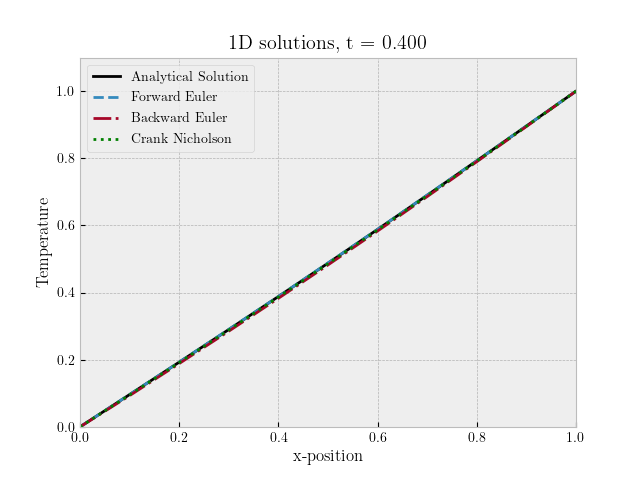
\includegraphics[width=0.95\linewidth]{./figures/plot1d0401.png}
	\caption{The three finite difference schemes, using $\dx = 0.1$, for a near steady state solution. The numerical schemes are plotted against the analytical solution. Also $\alpha = 0.5$, is the forced condition such that $\dt = \alpha\dx^2$.}
	\label{fig plot1d0401}
\end{figure}
\begin{figure}
	\centering
	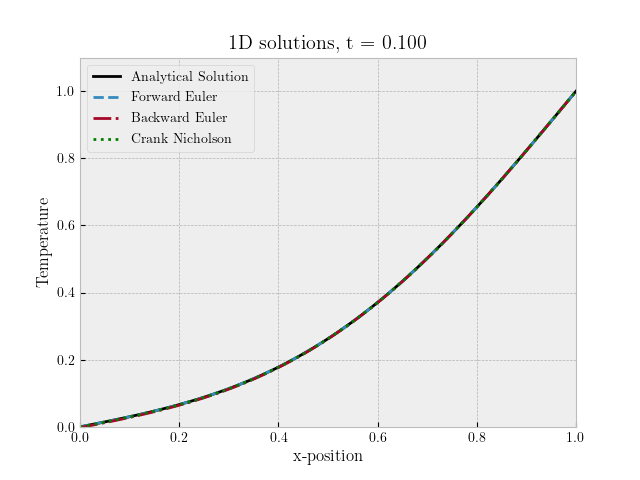
\includegraphics[width=0.95\linewidth]{./figures/plot1d01001.png}
	\caption{The three finite difference schemes, using $\dx = 0.01$, for a curved solution. The numerical schemes are plotted against the analytical solution. Also $\alpha = 0.5$, is the forced condition such that $\dt = \alpha\dx^2$.}
	\label{fig plot1d01001}
\end{figure}
\begin{figure}
	\centering
	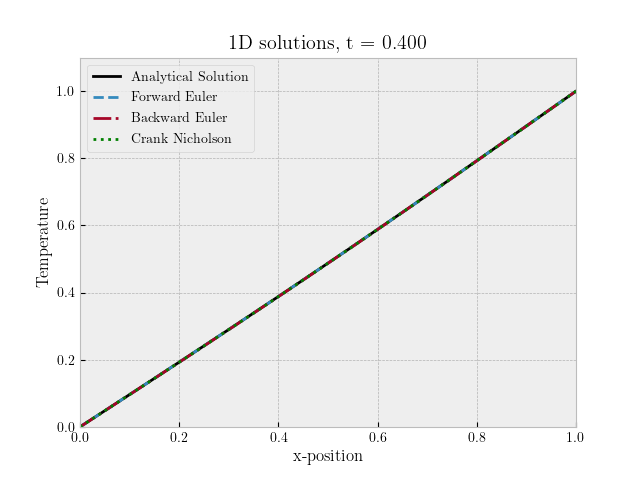
\includegraphics[width=0.95\linewidth]{./figures/plot1d04001.png}
	\caption{The three finite difference schemes, using $\dx = 0.01$, for a near steady state solution. The numerical schemes are plotted against the analytical solution. Also $\alpha = 0.5$, is the forced condition such that $\dt = \alpha\dx^2$.}
	\label{fig plot1d04001}
\end{figure}
\begin{figure}
	\centering
	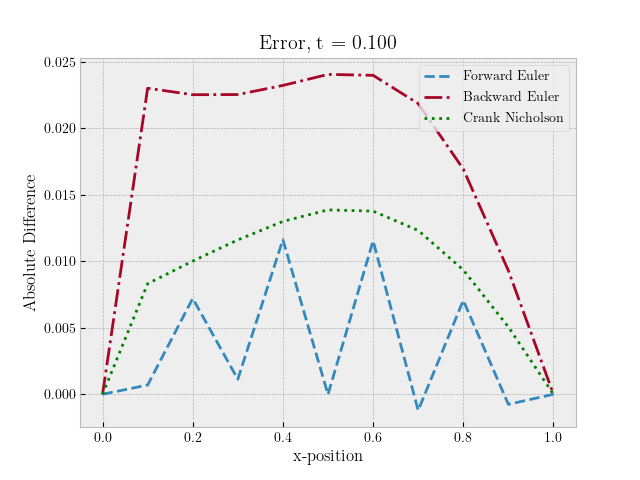
\includegraphics[width=0.95\linewidth]{./figures/error0101.png}
	\caption{The absolute error between the analytical solution and the numerical solutions. It is shown as the difference between the solutions, using $\alpha = 0.5$, and $\dx = 0.1$, up to t = 0.1.}
	\label{fig error0101}
\end{figure}
\begin{figure}
	\centering
	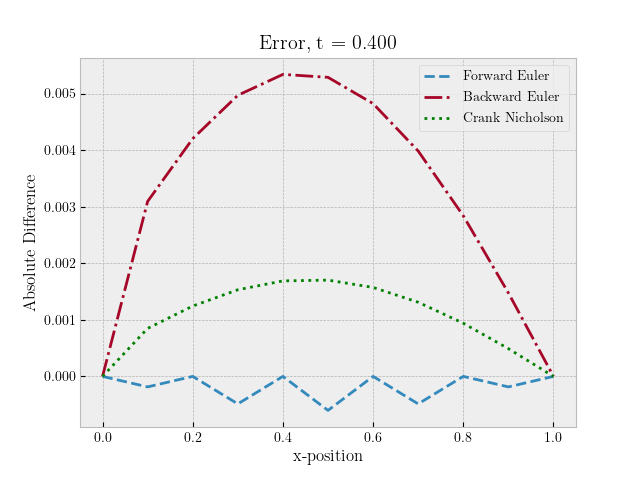
\includegraphics[width=0.95\linewidth]{./figures/error0401.png}
	\caption{The absolute error between the analytical solution and the numerical solutions. It is shown as the difference between the solutions, using $\alpha = 0.5$, and $\dx = 0.1$, up to t = 0.4.}
	\label{fig error0401}
\end{figure}
\begin{figure}
	\centering
	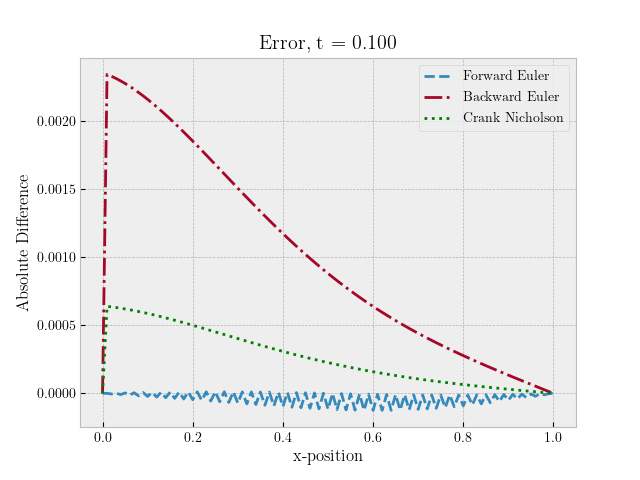
\includegraphics[width=0.95\linewidth]{./figures/error01001.png}
	\caption{The absolute error between the analytical solution and the numerical solutions. It is shown as the difference between the solutions, using $\alpha = 0.5$, and $\dx = 0.01$, up to t = 0.1.}
	\label{fig error01001}
\end{figure}
\begin{figure}
	\centering
	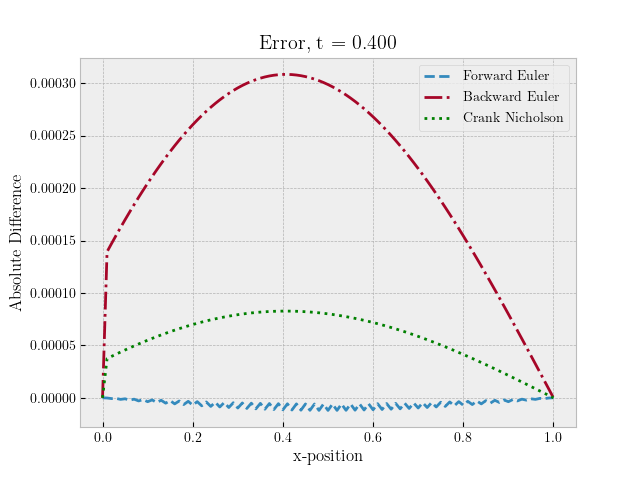
\includegraphics[width=0.95\linewidth]{./figures/error04001.png}
	\caption{The absolute error between the analytical solution and the numerical solutions. It is shown as the difference between the solutions, using $\alpha = 0.5$, and $\dx = 0.01$, up to t = 0.4.}
	\label{fig error04001}
\end{figure}

\begin{figure}
	\centering
	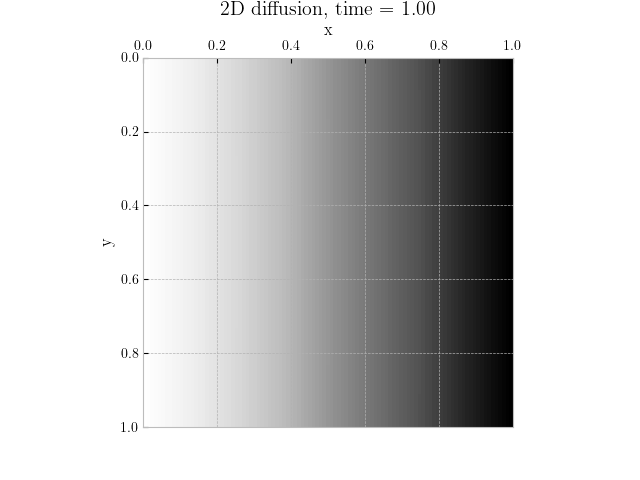
\includegraphics[width=0.95\linewidth]{./figures/2D1.png}
	\caption{The two-dimensional solution for the near steady state at t = 1. This is using the quasi one-dimensional solution approach and only depicts the numerical solution.}
	\label{fig 2d1}
\end{figure}
\begin{figure}
	\centering
	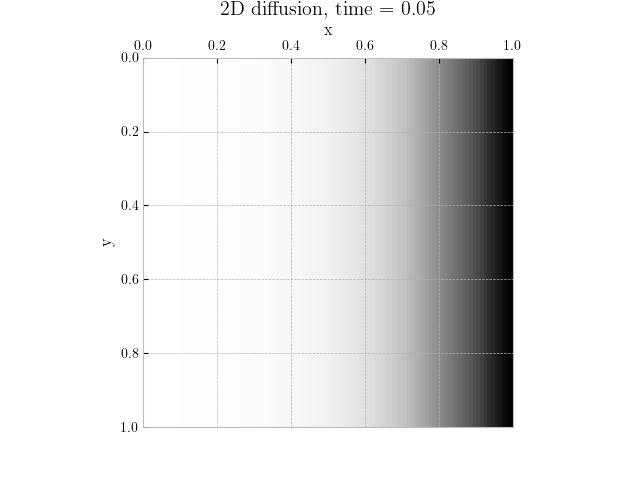
\includegraphics[width=0.95\linewidth]{./figures/2D2.png}
	\caption{The two-dimensional solution at t = 0.05, showing a curved solution, with large areas being near equal and a sharp peak. This is the same as we seen in \autoref{fig plot1d01001}.}
	\label{fig 2d4}
\end{figure}
\begin{figure}
	\centering
	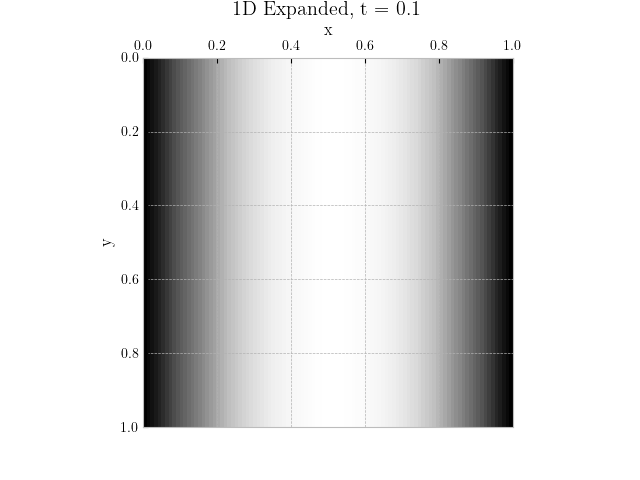
\includegraphics[width=0.95\linewidth]{./figures/2D1DExpand.png}
	\caption{The two-dimensional solution for $v(x,y,t)$, using the quasi one-dimensional approach. Showing what resembles a sine wave, which is expected from our one dimensional analytical solution.}
	\label{fig 2d2}
\end{figure}
\begin{figure}
	\centering
	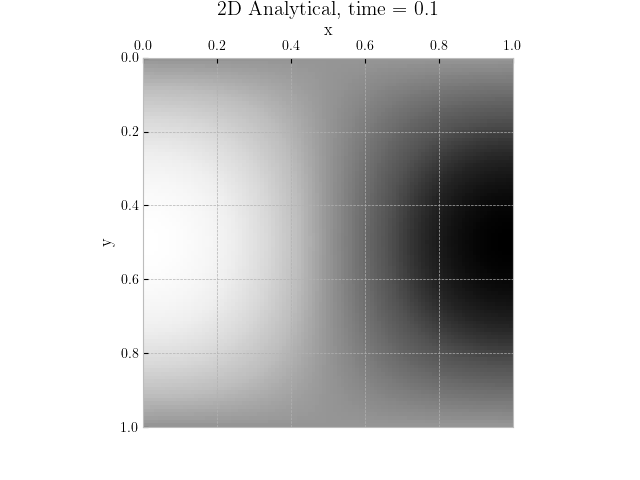
\includegraphics[width=0.95\linewidth]{./figures/2DAna.png}
	\caption{The two-dimensional closed-form solution, plotted in the same way as above. This is not what we expected as a result, and shows one peak and a through with fixed edges. }
	\label{fig 2d3}
\end{figure}



\section{Discussion} %0
\subsection{One-Dimension}
The one-dimensional case is a good stepping stone for the implementation of the algorithms and studying the system evolution. Including it can serve as a stepping stone to analysis of certain two-dimensional problems where they can be turned into a quasi one-dimensional problem. One such case is studying systems that have zero flux at the edges. 
\subsubsection{Methods}
An important part when choosing what numerical scheme to apply to a certain problem, a mixture between speed of implementation and correctness is desirable. As more complex methods such as the Crank-Nicholson or going further such as Runge-Kutta4 or similar, the implementation time is significantly longer than that of the forward Euler especially if no premade program can be used. And even in some cases, they have a quicker convergence and are more accurate than their counterparts. 

In \autoref{fig plot1d0101} we can see that the forward Euler is the method closest to that of the analytical solution in black. The backward Euler is furthest from the analytical solution, whilst the Crank-Nicholson strikes a middle ground between the two schemes. 
Not much more can be deduced from the plots over the solutions themselves, as the naked eye is not able to see the difference between the solutions. 
\subsubsection{Error}
As we can not deduce any noticeable difference between the schemes in the data plots themselves, by studying the absolute error we can see how the different methods behave compared to the analytical solution. These results can be seen in \autoref{fig error0101}, \autoref{fig error01001}, \autoref{fig error0401} and \autoref{fig error04001}. What we can see is a consistent trend of the forward Euler converging the quickest to the analytical solution, and with the decrease time steps seen in \autoref{fig error01001} and \autoref{fig error04001}, that the forward Euler is almost linear in shape. 
Only small fluctuations and a small curve is visible compared to its counterparts. 

The backward Euler is by far the worst when it comes to convergence and is far off the analytical solution in comparison to the forward Euler and would be a less than ideal scheme to apply for this problem. Even thought the scheme is stable for all choices of $\dt$ and $\dx$ it comes at a cost, that the scheme tends to become more inaccurate with larger choices of $\dt$ and $\dx$. 

The Crank-Nicholson strikes the middle ground again, whilst slower computationally than backward and forward Euler, it has a time truncation error of $\mathcal{O}(\dt^2)$. This would prove to be the superior choice for longer time simulations, where the stable solution is not reached quickly. 


\subsubsection{Methods Revisited}
After studying the error of the different methods, we can conclude that even though the forward Euler has a worse time accuracy than the Crank-Nicholson scheme, it converges significantly quicker and has a smaller error at the selected time steps. And for problems of a smaller size, especially scaled, using the forward Euler could be the best choice. However if you want to study larger systems over longer time scales, using schemes that are more accurate in time is beneficial even tough they come at a computational cost. As the Crank-Nicholson scheme, combines both the backward Euler and forward Euler. 

\subsection{Two-Dimensions}
The study of a two-dimensional problem, which has insulated edges is not always the most interesting, whilst having multiple real world applications, even a three dimensional problem, where you only have two edges for which you have any interaction with the area in question can be narrowed down to a simple one dimensional solution. Its counterpart is studying two-dimensional problems where you have different boundary conditions and perhaps different properties within the area in question.

From our study, we see that our two-dimensional case, in fact produces the same results as our one-dimensional case, which was what we expected. Furthermore from \autoref{fig 2d4}, we actually have what we can assume to be the exact same behavior as for our one-dimensional case. This is what we would expect from our boundary conditions as we have no flux at the edges. 

It would need more numerical study to ensure that the forward Euler in both cases, produces the same answers, however we can conclude that our results for studying a two-dimensional case with no fluxes at the edges can be simplified to a study of a quasi one-dimensional problem. 

\subsubsection{Quasi One-Dimensional}
As the boundary conditions for our two-dimensional problem is chosen such that there is no flux along the edges, we are dealing with a quasi one-dimensional problem, thus we can adapt our one-dimensional solution to also work for two-dimensions. This is because there are no changes in the $y$-direction and thus we have a problem where we are simply studying a one-dimensional problem in two-dimensions. 

Our one-dimensional solution can then be used as a baseline for the two-dimensional closed-form solution, to understand whether the solution we found is correct. From this we can see that in \autoref{fig 2d3} is far from what is expected as seen in \autoref{fig 2d2} and some part of our two-dimensional closed-form solution or implementation is incorrect. 

\subsubsection{Analytical Solution}
The study of the two-dimensional problem is based on the quasi one-dimensional approach, instead of using our closed-form two-dimensional solution. This is because as stated we our closed-form two-dimensional solution is not producing the results as expected. We observe a pattern in \autoref{fig 2d3} that is similar to that of a peak and a through with fixed boundary values which is not what we seen in \autoref{fig 2d2}, which is resembles a wave with troughs on either side and a peak in the middle which is expected of a sine wave. The reason for the disagreement between our quasi one-dimensional solution and the two-dimensional analytical solution could be due to different factors.  

The first, our closed-form solution may be wrong, and would never produce the results which we expect to see. However no such errors has been found when proof reading the solution, and it is left in as the closed-form solution to the two-dimensional problem. 

The second, could be that our implementation of the double Fourier-series is wrong. This is equally likely to be the case, and no solution or improvement to the implementation that would result in the expected results was found. 

\section{Conclusion} %0
We have reviewed different finite difference schemes, studying their mathematical truncation error and stability for solving the diffusion equation in one and two spatial dimensions. Establishing functional numerical methods for both dimensions, in agreement with our one-dimensional solutions and quasi one-dimensional solutions. We found that the convergence of the forward Euler is significantly faster than both the implicit schemes. No study of the stability conditions, i.e. the constraint put on $\dt$ and $\dx$ was done. Instead the choice of $\dt$ and $\dx$ where made such that we always had $\alpha = 0.5$ for the one-dimensional case and $\alpha = 0.25$ for the two-dimensional case. Whilst the forward Euler has a quicker convergence, both the implicit schemes have no restrictions on their choices of $\dt$ and $\dx$, and the Crank-Nicholson scheme having the best truncation error in the time dimension. This makes the Crank-Nicholson scheme, even though computationally expensive, the best choice for solving the diffusion equation. In two-dimensions we only developed the explicit scheme which reproduced the expected results from our assumptions of the setup problem. Reproducing the quasi one-dimensional problem we had, however we were not able to reproduce the correct results with our analytical solution. Either due to poor implementation or wrong closed-form solution, the solution found for the two-dimensional problem did not reproduce the numerical results that supported our expectation. Further study of the accuracy of the two-dimensional case and in-depth study of the stability of the different schemes in one-dimension. A further study of more advanced implicit methods in the two-dimensional case.

\bibliography{bib_proj5}
\bibliographystyle{IEEEtran}


\appendix
\section{Analytical Solution for Two Dimensions}\label{app 2DA}
To find the analytical solution of equation \eqref{eq diffusion 2d}, we start off with separation of variables
\begin{equation}
	u(x,y,t) = X(x)Y(y)T(t).
\end{equation}
Inserting in the original PDE we get 
\begin{equation}
	\frac{T'(t)}{T(t)} = \frac{X''(x)}{X(x)} + \frac{Y''(y)}{Y(y)}.
\end{equation}
Since the l.h.s. depend on t and the r.h.s. on $(x,y)$, both sides must equal a constant $-\lambda$. Such that we have 
\begin{equation}\label{eq 2d speration}
	\begin{split}
		\frac{T'(t)}{T(t)} &= -\lambda \\
		\frac{X''(x)}{X(x)} + \frac{Y''(y)}{Y(y)}&= -\lambda 
	\end{split}
\end{equation}


Our boundary and initial conditions are as before, given by 
\begin{equation}
	\begin{split}
		u(0,y,t) = 0, &\quad \fracpy u(x,0,t) = 0\\
		u(L,y,t) = 0, &\quad \fracpy u(x,L,t) = 0\\
		u(x,y,0) &= f(x,y)
	\end{split}
\end{equation}
where we have $f(x,y) = -x/L$. This can be found the same way as for the one dimensional case, and as we have no variance in the $y$-direction, due to studying a quasi one dimensional problem, this equations holds for $f(x,y)$.

From equation \eqref{eq 2d speration}, we have that 
\begin{equation}
	T(t) = C_1 e^{-\lambda t}
\end{equation}
Separating the boundary conditions we have that 
\begin{align*}
	u(0,y,t) = 0 &\implies X(0) = 0\\
	u(L,y,t) = 0 &\implies X(L) = 0\\
	\fracpy u(x,0,t) = 0 &\implies Y'(0) = 0\\
	\fracpy u(x,L,t) = 0 &\implies Y'(L) = 0
\end{align*}

Rearranging the spatial part of the equation gives 
\begin{equation}
	\frac{Y''(y)}{Y(y)} + \lambda = -\frac{X''(x)}{X(x)}.
\end{equation}
Since the l.h.s. depends on $y$ and the r.h.s. depends on $x$, both sides must again equal a constant, say $\mu$,
\begin{equation}
	\frac{Y''(y)}{Y(y)} + \lambda = -\frac{X''(x)}{X(x)} = \mu.
\end{equation}
This gives us 
\begin{equation}
	X''(x) + \mu X(x) = 0, \quad X(0) = 0 = X(L),
\end{equation}
for which solution is the same as the one for one dimension, namely 
\begin{equation}
	X_n(x) = \sin\left(\frac{n\pi x}{L}\right), \quad \mu_n = \left(\frac{n\pi}{L}\right)^2
\end{equation}
for $n=1,2,3,\dots$.

For $Y(y)$, we on the other hand have 
\begin{equation}
	Y''(y) + \left(\lambda - \mu_n\right)Y(y)=0, \quad Y'(0) = 0 = Y'(L)
\end{equation}
which have the following solution
\begin{equation}
	Y_m(y) = \cos\left(\frac{m\pi y}{L}\right), \quad \left(\lambda_{nm} - \mu_n\right) = \left(\frac{m\pi}{L}\right)^2
\end{equation}
for $m=1,2,3,\dots$. 

Which then gives us the general solution as 
\begin{equation}
	u(x,y,t) = \sin\left(\frac{n\pi x}{L}\right)\cos\left(\frac{m \pi y}{L}\right)e^{-\lambda_{nm}t}
\end{equation}
for $m,n = 1,2,3,\dots$. Giving us a set of solutions given by 
\begin{equation}
	u(x,y,t) = \sum_{m=1}^\infty\sum_{n = 1}^\infty A_{nm}u_{nm}
\end{equation}
Where $A_{nm}$, is given by 
\begin{equation}
	A_{nm} = \frac{4}{L^2}\int_{x=0}^{L}\int_{y=0}^{L}f(x,y)\sin\left(\frac{n\pi x}{L}\right)\cos\left(\frac{m \pi y}{L}\right)dy\,dx.
\end{equation}

\end{document}
